\chapter{Introducción}
\label{cap:capitulo1}
\setcounter{page}{1}

Desde sus inicios, la robótica ha proporcionado un sinfin de posibilidades y alternativas ante problemas que anteriormente carecían de las soluciones adecuadas, pero, ¿qué es realmente la robótica?\\

Se podría definir \textit{robótica} como el proceso mediante el cual una máquina intercambia energía e información con su entorno, con el propósito de alcanzar una serie de objetivos específicos. Este campo tecnológico en expansión es el resultado de décadas de colaboración contínua entre biólogos, informáticos e ingenieros \cite{Koditschek21}.

Dada esta multidisciplina, la robótica abarca una amplia gama de aplicaciones, desde la industria hasta la medicina, pasando por la exploración espacial, la domótica o la conducción autónoma, entre otras. Es un campo en constante evolución, impulsado por la búsqueda de soluciones innovadoras para mejorar la calidad de vida y permitir superar desafíos de manera más eficiente y segura.\\

La industria agrícola no es una excepción, ya que ha contemplado históricamente tareas que requieren una dedicación laboral considerable. No obstante, gracias a la robótica y a los sistemas de visión artificial, surge la oportunidad de transformar una serie de procesos, como puede ser la recolección de cultivos, a través de la detección automatizada para su posterior recolección.\\

En las siguientes secciones describiremos brevemente algunas de las aplicaciones más importantes de la robótica en la sociedad actual, así como los distintos conceptos en los cuales se basa la investigación y el desarrollo llevado a cabo.\\

\section{Robots y robótica}
\label{sec:robótica} % etiqueta para luego referenciar esta sección

Según la Federación Internacional de Robots (IFR) se define robot según el vocabulario establecido por la International Organization for Standardization (ISO), y esto es como \textit{"mecanismo accionado programado con cierto grado de autonomía para realizar tareas de locomoción, manipulación o posicionamiento"} \cite{ISO8373}.\\  

El término \textit{“robot”} fue utilizado por primera vez por Karel Capek (en su obra de teatro “Rossum’s Universal Robots” publicada en 1920. Esta palabra viene del vocablo checo \textit{“robota”} que significa “trabajo”, en el sentido de la obligatoriedad, entendido como servidumbre, trabajo forzado o esclavitud \cite{Sanchez07a}.

Aunque esta definición es un punto de partida, es cierto que es posible diferir en aspectos como si un robot debe controlarse automáticamente o podría ser autónomo o si un robot debe ser reprogramable. A un nivel más amplio, cualquier máquina que pueda utilizarse para llevar a cabo acciones o tareas complejas de forma automática puede considerarse un robot \cite{Raj19}.\\

Históricamente, las civilizaciones antiguas, como la egipcia y la griega, dieron los primeros pasos en lo que se puede denominar \textit{robótica clásica}, construyendo autómatas y mecanismos diseñados para imitar acciones humanas, con características mecánicas rudimentarias. 
Con el paso del tiempo, la ciencia y la ingeniería avanzaron, y los conceptos de la robótica comenzaron a tomar forma más definida hasta que, en el siglo XX, con el desarrollo de la ingeniería en sus diferentes ramas (mecánica, electrónica, informática, telecomunicaciones), \textbf{\emph{Isaac Asimov}} (1920-1992) utilizó por primera vez el término \textit{“robótica”} y postuló las tres leyes de la robótica en su libro \textit{I Robot} publicado en 1950, coincidiendo con el apogeo de la \textit{robótica moderna}. Asimov consideró necesario añadir una cuarta ley, antepuesta a las demás, la número cero, que afirma que un robot no debe actuar simplemente para satisfacer intereses individuales, sino que sus acciones deben preservar el beneficio común de toda la humanidad \cite{Sanchez07b}.

\pagebreak

\begin{table} [h!]
  \begin{center}
    \begin{tabular}{p{15cm}} % Ajustar el ancho según necesidades
      \hline
      1. Un robot no debe dañar a un ser humano ni, por su pasividad, dejar que un ser humano sufra daño.\\\\
    
      2. Un robot no debe obedecer las órdenes que le son dadas por un ser humano, excepto cuando estas órdenes están en oposición con la primera Ley.\\\\
    
      3. Un robot debe proteger su propia existencia, hasta donde esta protección no esté en conflicto con la primera o segunda Ley. \\
      \hline
    \end{tabular}
  \end{center}
  \caption{Las tres leyes de la robótica según Asimov.}
  \label{cuadro:leyesrobotica_Asimov}
\end{table}

Es también en 1950, cuando \textbf{\emph{Alan Mathison Turing}} publica \textit{“Computing Machinery and Intelligence”} y propone una prueba (test o máquina de Touring), en forma de entidad matemática abstracta, que demuestra la existencia de problemas computacionales irresolubles que ninguna máquina es capaz de solventar. Se puede afirmar que un programa de ordenador no llegará nunca a ser tan inteligente como un ser humano y que un robot no podrá suplir al ser humano de forma completa, \cite{Sanchez07b} preocupación sobre el potencial de sustitución de la mano de obra, que históricamente, ha atenuado el entusiasmo en torno a las nuevas tecnologías \cite{Mokyr15}.\\

Partiendo de todos estos avances y del interés por automatizar las tareas de producción, la robótica va adquiriendo un gran desarrollo \cite{Sanchez07b}. Es debido a este desarrollo, que atendiendo al propósito y al contexto en el que se utilicen estos robots, se fueron creando varios grupos en función de los que clasificarles. Estos tres grandes grupos en función de una serie de criterios generales fueron: \textit{robots industriales}, \textit{robots de servicio} y \textit{robots médicos}.

\pagebreak

\subsection{Robot Industrial}
\label{sec:robot_industrial}

Se define \textit{robot industrial} como un "manipulador polivalente, reprogramable y controlado automáticamente, programable en tres o más ejes, que puede ser fijo o móvil para su uso en aplicaciones de automatización industrial" \cite{ISO8373}.\\

El inicio de la robótica industrial, tal como la definimos actualmente, puede datarse en la década de 1950, aunque algunos tipos de automatización en el entorno industrial empezaron a aparecer desde los tiempos de la Revolución Industrial. La evolución de los robots industriales puede subdividirse en cuatro categorías: las tres primeras abarcan el período comprendido entre los años cincuenta y finales de los noventa, mientras que la cuarta generación abarca desde 2000 hasta nuestros días \cite{Gasparetto19}.

\begin{itemize}
  \item \textit{Primera generación o primeros manipuladores (1950-1967):} Estos robots eran básicamente máquinas programables que no tenían comunicación con el entorno externo y con algoritmos de control sencillos (punto a punto). En cuanto al hardware, contaban con equipos de baja tecnología, sin servocontroladores. Sin embargo, en 1954, \textbf{\emph{George Devol}} y \textbf{\emph{Joseph Engelberger}} formaron la empresa \emph{Unimation}, empresa que desarrollaría \textbf{\emph{Unimate}}, considerado el primer robot industrial de la historia, fabricado en 1961 \cite{Zamalloa17}.
  
  \begin{figure}[h!]
    \begin{center}
      \subcapcentertrue
      \subfigure[Joseph Engelberger y George Devol]{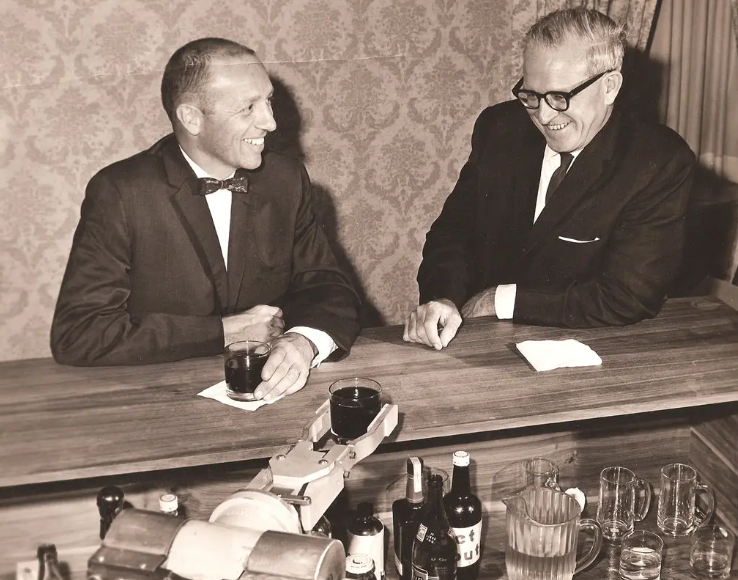
\includegraphics[width=62mm]{figs/Engelberger_Devol.png}}
      \hspace{2mm}
      \subfigure[Robot Unimate]{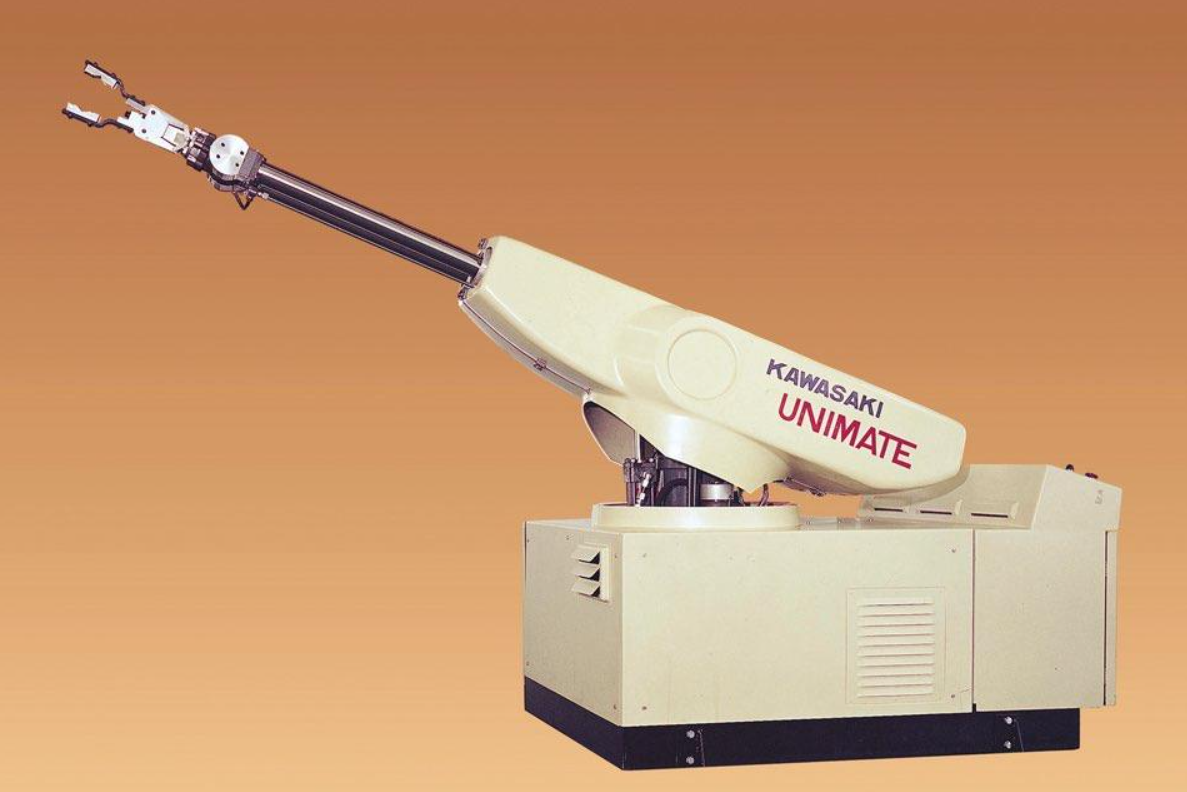
\includegraphics[width=73mm]{figs/Unimate robot.png}}
    \end{center}
    \caption{Primer robot industrial.}
    \label{fig:primer_robot_industrial}
  \end{figure}
  
  \pagebreak
  
  Empresas como \emph{Ford} y \emph{General Motors} empezaron a plantearse la automatización de sus plantas productivas, por lo que, en 1962, la empresa \emph{AMF Corporation} fabricó un nuevo robot llamado \textit{Versatan}, un robot cilíndrico que \emph{Ford} encargó para sus fábricas.
Este robot, fue también el primero que se instaló en un centro productivo en Japón \cite{Gasparetto19}. 

  \item \textit{Segunda generación o robots sensorizados (1968-1977):} eran máquinas programables básicas con posibilidades limitadas de comportamiento autoadaptativo y capacidades elementales para reconocer el entorno externo, poseían sistemas sensoriales avanzados y eran robots de gran volumen que se utilizaban principalmente en automoción \cite{Zamalloa17}.

  En 1968, en el Stanford Artificial Inteligente Laboratory (SRI) se confecciona el WAVE, el primer lenguaje de programación para robots. También en el mismo centro surge \emph{Shakey}, provisto de múltiples sensores y medios para desplazarse por el suelo, además de control remoto por radio \cite{Sanchez07b}.
  
  \begin{figure} [h!]
    \begin{center}
      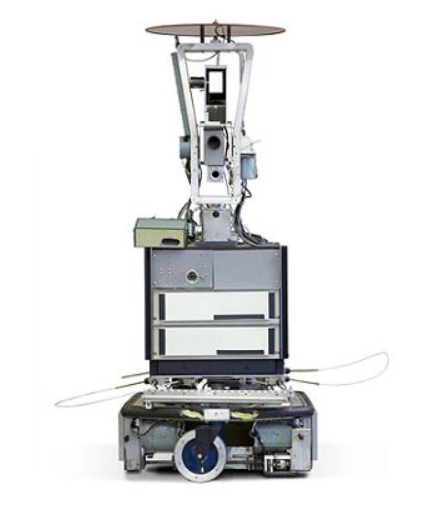
\includegraphics[width=8cm]{figs/Shakey.png}
    \end{center}
    \caption{Robot Shakey.}
    \label{fig:shakey}
  \end{figure}

  Shakey podía realizar tareas de planificación, búsqueda de rutas y reordenación de objetos sencillos, siendo el primer robot móvil con capacidad para percibir y razonar sobre su entorno \cite{sri}.
  
  \pagebreak
  
  En 1969, \emph{Unimation} concendió a \emph{Kawasaki Heavy Industries Ltd.} la licencia para producir robots para el mercado japonés y asiático,    		conduciendo al desarrollo del Kawasaki-Unimate 2000, el primer robot industrial construido en Japón. Es también en este año cuando \textbf{\emph{Víctor Scheinman}}, un estudiante de ingeniería mecánica de la Universidad de Standford, diseñó y construyó el primer prototipo de brazo robótico, cuya cinemática inversa podía resolverse de manera analíticamente cerrada, permitiendo una rápida ejecución de la trayectoria \cite{Gasparetto19}. 

  \begin{figure}[h!]
    \begin{center}
      \subcapcentertrue
      \subfigure[Victor Scheinman con el Standford Arm]{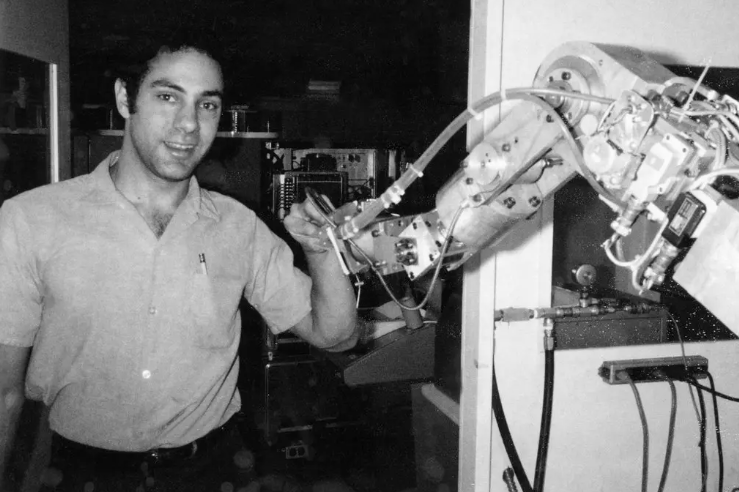
\includegraphics[width=62mm]{figs/Victor_Scheinman.png}}
      \hspace{2mm}
      \subfigure[Standford Arm]{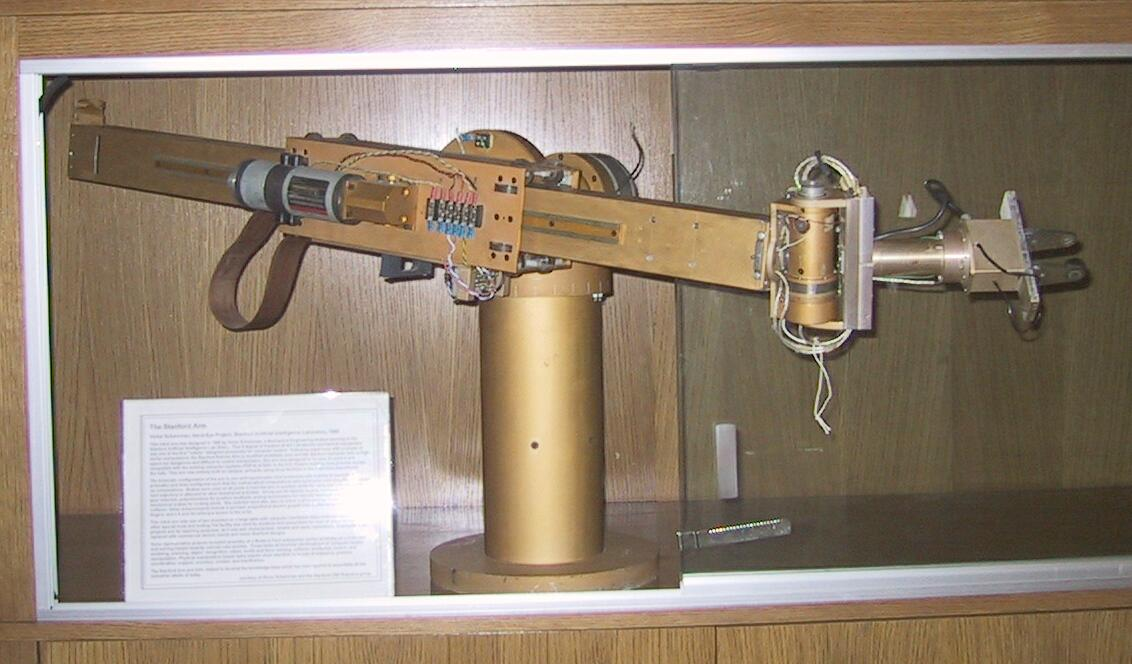
\includegraphics[width=71mm]{figs/Standford_arm.jpeg}}
    \end{center}
    \caption{Standford Arm.}
    \label{fig:standford_arm}
  \end{figure}

  El ingeniero de la compañía \emph{Yaskawa}, \textbf{\emph{T Mori}}, en 1969 acuña el término \emph{mecatrónica} que integra el conjunto de mecanismos de control automático imprescindibles para el desarrollo de cualquier máquina inteligente \cite{Sanchez07b}.
  
  \begin{figure} [h!]
    \begin{center}
      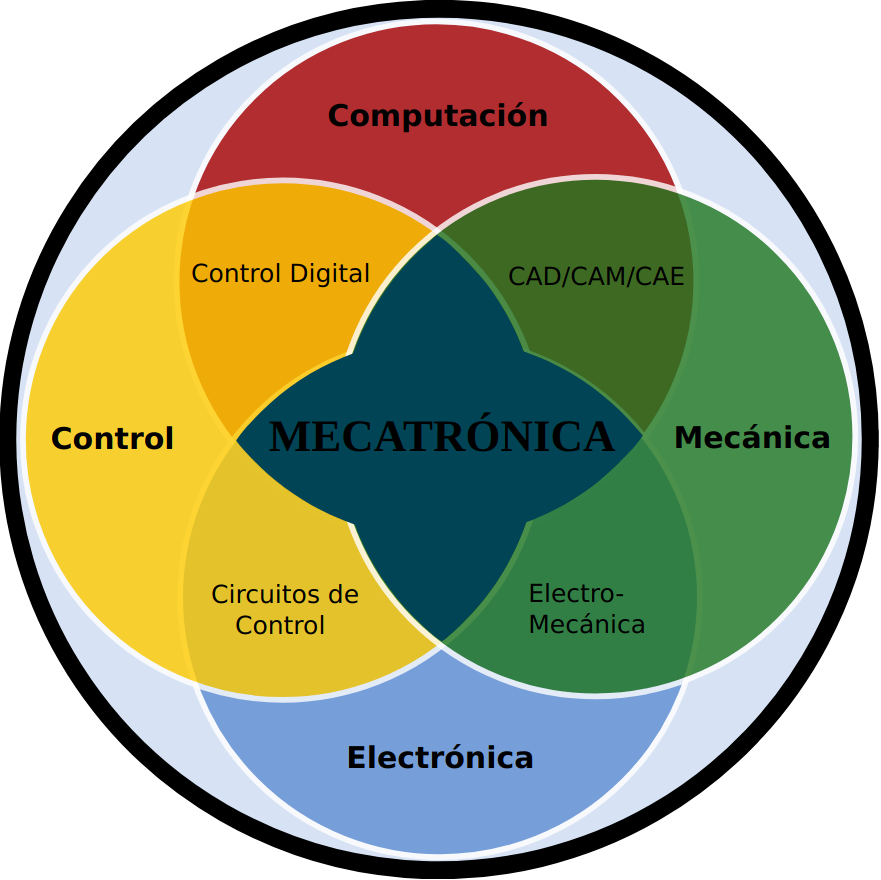
\includegraphics[width=65mm]{figs/meca.png}
    \end{center}
    \caption{Diagrama mecatrónico de construcción de máquinas inteligentes.}
    \label{fig:Mecatrónica}
  \end{figure}
  
  \pagebreak

  En 1973, \emph{KUKA} construyó el primer robot industrial con 6 ejes electromecánicos llamado Famulus. Un año más tarde, \emph{Cincinnati Milacron} introdujo en el mercado el robot T3. Cincinnati Milacron (adquirida por \emph{ABB} en 1990). El robot T3 fue el primer robot comercial controlado por un microordenador \cite{Zamalloa17}.
  
  \begin{figure} [h!]
    \begin{center}
      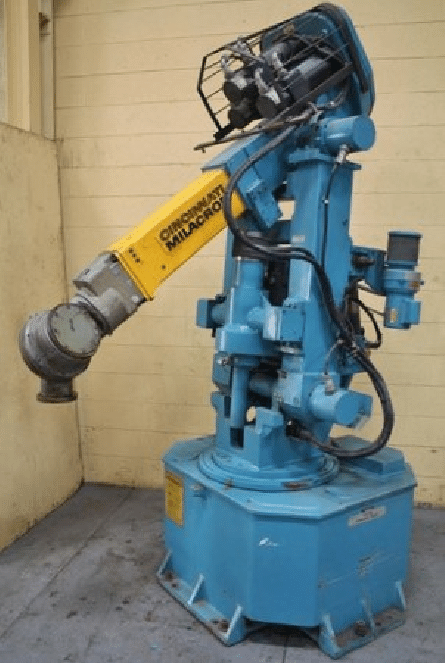
\includegraphics[width=55mm]{figs/T3_robot.png}
    \end{center}
    \caption{Cincinnati Milacron T3 robot.}
    \label{fig:T3}
  \end{figure}
  
  \item \textit{Tercera generación o robots industriales (1978-1999):} los robots de esta generación disponían de controladores específicos (ordenadores), siendo un punto clave en la caracterización de este generación, además del surgimiento de nuevos lenguajes de programación para el control de los robots, la posibilidad de reprogramarlos y la inclusión parcial de la visión artificial \cite{Zamalloa17}.
  
  Entre finales de los años setenta y principios de los ochenta, otros avances científicos y técnicos contribuyeron a la difusión de los robots \cite{Gasparetto19}, que junto a que las empresas de todo el mundo invirtieron miles de millones de dólares en del mundo para automatizar tareas básicas en sus cadenas de montaje, supusieron que los robots poblaran muchos sectores industriales para automatizar una amplia variedad de actividades \cite{Zamalloa17}.
  
  Unimation diseñó y fabricó en 1978 el robot PUMA. El PUMA (acrónimo de Programmable Universal Machine for Assembly) fue considerado durante muchas décadas el arquetipo de los robots antropomórficos \cite{Gasparetto19}.\\
  
  En 1978, el científico japonés \textbf{\emph{Hiroshi Makino}}, de la Universidad de Yamanashi, propuso una nueva estructura cinemática. El robot con esta estructura se denominó \emph{SCARA} (acrónimo de "Selective Compliance Assembly Robot Arm"), ya que su conformidad en la dirección horizontal resultó menor que la conformidad en la dirección vertical. Por esta razón, así como por la ligereza de la cadena cinemática (que permitía un controlador más sencillo y rápido), este robot era adecuado para ser empleado en tareas como el ensamblaje de objetos pequeños \cite{Makino80}.
  
  \begin{figure} [h!]
    \begin{center}
      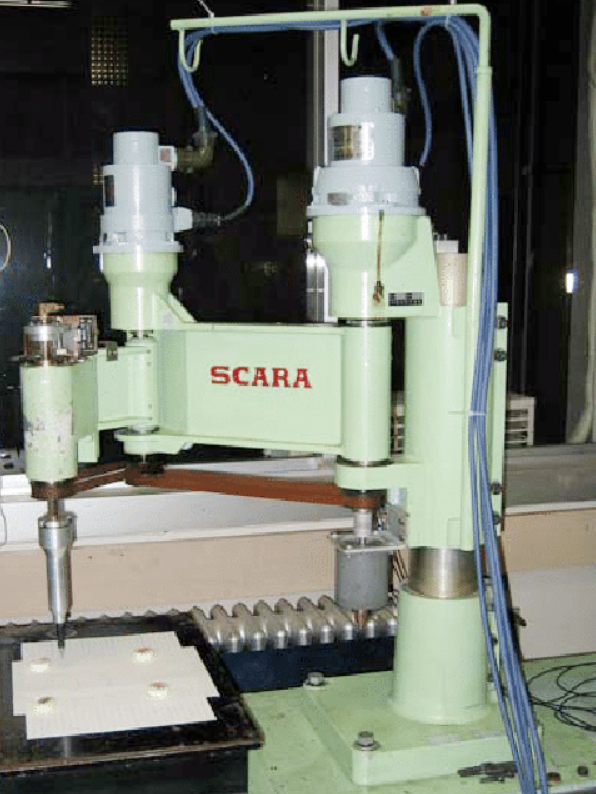
\includegraphics[width=55mm]{figs/Scara.png}
    \end{center}
    \caption{Uno de los primeros prototipos de robot SCARA.}
    \label{fig:Scara}
  \end{figure}
  
  Más tarde, en 1981 en la Universidad Carnegie-Mellon se desarrolló un robot de impulsión directa que utiliza motores eléctricos en las articulaciones, evitando la distorsión de las transmisiones mecánicas convencionales. En 1982 \emph{IBM} introduce el robot de montaje industrial RS-1 que utiliza un brazo constituido por 3 dispositivos de deslizamiento \cite{Sanchez07b}.

\end{itemize}\

\subsection{Robot de Servicio}
\label{sec:robot_servicio}

Se define \textit{robot de servicio} como un robot que realiza tareas útiles para las personas o los equipos, incluyendo en esta la manipulación o el servicio de artículos, el transporte, el apoyo físico, la orientación o información, el aseo personal, la cocina y la manipulación de alimentos y la limpieza en el ámbito personal, y la inspección, vigilancia, manipulación de objetos, transporte de personas, orientación o información, cocina y manipulación de alimentos y limpieza en el ámbito profesional \cite{ISO8373}.
 

\subsection{Robot Médico}
\label{sec:robotica_industrial} 

Se define \textit{robot médico} a aquellos dispositivos electromecánicos que desempeñan parcial o totalmente algunas funciones de los seres humanos o de sus órganos al resolver problemas médicos, ayudando a mejorar la asistencia al paciente y los resultados, a la vez que aumenta la eficiencia operativa \cite{Kraevsky10}.\\

En los textos puedes poner palabras en \textit{cursiva}, para aquellas expresiones en sentido \textit{figurado}, palabras como \textit{robota}, que está fuera del diccionario castellano, o bien para resaltar palabras de una colección: \textit{(a)} es la primera letra del abecedario, \textit{(b)} es la segunda, etc.\\

Al poner las dos líneas del anterior párrafo, este aparecerá separado del anterior. Si no las pongo, los párrafos aparecerán pegados. Sigue el criterio que consideres más oportuno.

\section{Segunda sección}
\label{sec:segundaseccion}

No olvides incluir imágenes y referenciarlas, como la Figura \ref{fig:roomba}.

\begin{figure} [h!]
  \begin{center}
    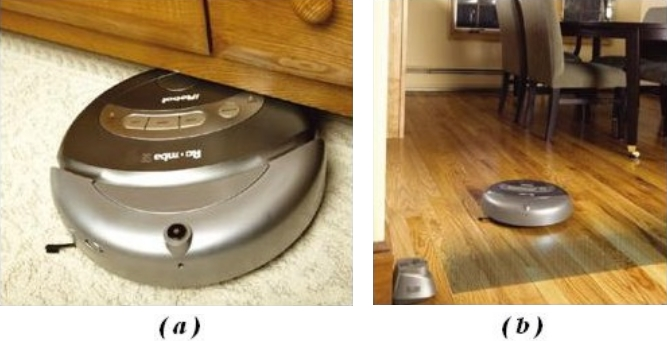
\includegraphics[width=8cm]{figs/roomba}
  \end{center}
  \caption{Robot aspirador Roomba de iRobot.}
  \label{fig:roomba}
\end{figure}\

Ni tampoco olvides de poner las URLs como notas al pie. Por ejemplo, si hablo de la Robocup\footnote{\url{http://www.robocup.org}}.

\subsection{Números}
\label{sec:subseccion}

En lugar de tener secciones interminables, como la Sección \ref{sec:miseccion}, divídelas en subsecciones.

Para hablar de números, mételos en el entorno \textit{math} de \LaTeX, por ejemplo, $1.5Kg$. También puedes usar el símbolo del Euro como aquí: 1.500\euro.

\subsection{Listas}

Cuando describas una colección, usa \texttt{itemize} para ítems o \texttt{enumerate} para enumerados. Por ejemplo:

\begin{itemize}
 \item \textit{Entorno de simulación.} Hemos usado dos entornos de simulación: uno en 3D y otro en 2D.
 \item \textit{Entornos reales.} Dentro del campus, hemos realizado experimentos en Biblioteca y en el edificio de Gestión.
\end{itemize}\

\begin{enumerate}
 \item Primer elemento de la colección.
 \item Segundo elemento de la colección.
\end{enumerate}\

\paragraph{Referencias bibliográficas}
\label{sec:referencias}

% Cita, sobre todo en este capítulo, referencias bibliográficas que respalden tu argumento. Para citarlas basta con poner la instrucción \verb|\cite| con el identificador de la cita. Por ejemplo: libros como \cite{vega12e}, artículos como \cite{vega19b}, URLs como \cite{vega19a}, tesis como \cite{vega18b}, congresos como \cite{vega18a}, u otros trabajos fin de grado como \cite{vega08b}.

Las referencias, con todo su contenido, están recogidas en el fichero \texttt{bibliografia.bib}. El contenido de estas referencias está en formato \texttt{BibTex}. Este formato se puede obtener en muchas ocasiones directamente, desde plataformas como \texttt{Google Scholar} u otros repositorios de recursos científicos.

Existen numerosos estilos para reflejar una referencia bibliográfica. El estilo establecido por defecto en este documento es APA, que es uno de los estilos más comunes, pero lo puedes modificar en el archivo \texttt{memoria.tex}; concretamente, cambiando el campo \verb|apalike| a otro en la instrucción \verb|\bibliographystyle{apalike}|. 

\

\

\

Y, para terminar este capítulo, resume brevemente qué vas a contar en los siguientes.
